All performance tests reported in this paper were conducted on the Cori system at NERSC. Cori Phase I is a Cray XC40 system with 1632 dual-socket compute nodes. Each node consists of two 2.3GHz 16-core Haswell processors and 128GB of DRAM. The Cray Aries high-speed interconnect is configured in a ``Dragonfly' topology. We use a Lustre scratch filesystem with 27PB of storage, and over 700 GB/s peak I/O performance. 

\paragraph{Spark Configuration.}
We use the Standalone Cluster Manager to run the Spark cluster. This is a collection of scripts that start the driver process and use ssh to start the executor processes on each node. Once the executors are started, they communicate with the driver via akka-tcp. When an application is submitted to the Spark cluster a second java process is spawned by each executor that controls the computation for that application. Sometimes this second process will fail to start and the executor does not participate in the calculation. The exact cause of this is not well known. Running Spark in an encapsulated Shifter image reduces the rate of these failures, which suggests this could be due to a race condition in the code.

\paragraph{H5Spark: Loading HDF5 data natively into Spark.}
The Daya Bay and climate data sets are stored in HDF5. We utilized the H5Spark~\cite{h5spark-cug16} package to read this data in as one RDD object. H5Spark provides a parallel I/O interface that efficiently loads TBs of data into the workers' memory and constructs a single RDD. An MPI-like independent I/O is performed in H5Spark to balance the workload. H5Spark partially relies on the Lustre file system striping to achieve high I/O bandwidth. We chose a Lustre configuration optimal for each data set: we stored the Daya Bay data on 72 OSTs and the climate data sets on 140 OSTs, both with striping size of 1MB. 

\paragraph{Shifter.}
Shifter is a framework that delivers docker-like functionality to HPC \cite{shifter}. It works by extracting images from native formats (such as a Docker image) and converting them to a common format that is optimally tuned for the HPC environment. %On Cori, users can pull down images directly from Docker or from other private registries and run this image on thousands of nodes simultaneously. This functionality is tied into the slurm batch system and requested images are automatically started at the beginning of jobs. 
Shifter allows users with a complicated software stack to easily install them in the environment of their choosing. It also offers considerable performance improvements because metadata operations can be more efficiently cached compared to a parallel file system and users can customize the shared library cache (ldconfig) settings to optimize access to their analysis libraries. In particular, shared library performance, which has long been a pain point on Cray systems, is dramatically improved. For this analysis we used two separate Shifter images. A generic ``CCM'' image which only contained SSH functionality (which is otherwise absent by default on Cray compute nodes) and a full “spark” image which contained version 1.5.1 of Spark  compiled with OpenBLAS \cite{openblas} and SSH. The Spark image is available on Docker Hub \cite{dockerspark}. 

\paragraph{Spark Tuning Parameters.}
Shifter provides a user-controlled option to create a writeable temporary space that is private to each node. This has performance characteristics similar to a local disk. This is created by mounting a writeable loop-back mounted file system which is backed by the parallel file system. This feature is very useful for frameworks like Spark that assume the presence of a local disk that can be used to store node local temporary files and spills. Metadata operations and small I/O transactions can  be more efficiently cached on the compute node since, unlike the Lustre scratch file system, it doesn't have to maintain coherency of this file system with other nodes. Most importantly, as the Spark cluster size is scaled up, this approach helps avoid additional pressure on the Lustre Metadata Servers which are the least scalable components of the file system. Since Spark opens and closes files many times, using the loop-back mounted file system as a writable cache can improve performance \cite{scalingspark16}.

We followed general Spark guidelines for Spark configuration values. The driver and executor memory were both set to 100 GB, a value chosen to maximize the memory available for data caching and shuffling while still leaving a buffer to hedge against running the nodes out of memory.  Generally we found that fetching an RDD from another node was detrimental to performance, so we turned off speculation (a function that restarts tasks on other nodes if it looks like the task is taking longer than average). We also set the spark locality wait to two minutes, this ensures that the driver will wait at least two minutes before scheduling a task on a node that doesn't have the task's RDD. The total number of spark cores was chosen such that there was a one-to-one correspondence between spark cores and physical cores on each node (with the exception of the 50-node NMF run which used a factor of two more partitions because it ran into hash table size issues). We used the KryoSerializer for deserialization of data. We compiled Spark to use multi-threaded OpenBLAS for PCA.

\paragraph{C+MPI Tuning Parameters.}
The NMF algorithm uses the Tall-Skinny QR (TSQR) \cite{ballard14,demmel12} factorization implemented as part of the Communication-Avoiding Dense Matrix Computations (CANDMC) library \cite{Solomonik14} which links to Intel MKL for optimized BLAS routines using the Fortran interface and ensured that loops were auto-vectorized when possible. We explored multi-threading options with OpenMP but found that it did not significantly improve performance. Applying TSQR on the Daya Bay data set results in a $192 \times 192$ upper-triangular matrix. Due to the small size we utilized a sequential non-negative least squares solver by Lawson and Hanson \cite{lawson95} in the \textsc{XRay} algorithm. PCA requires EVD, SVD, matrix-vector products, and matrix-matrix products. We use arpack-ng \cite{Lehoucq97} for the SVD and link to single-threaded Cray LibSci for optimized BLAS routines using the C interface. All experiments were conducted using a flat-MPI configuration with one MPI process per physical core and disabled TurboBoost.

\paragraph{Spark Overheads.}
To report the overheads due to Spark's communication and synchronization costs, we group them into the following bins, illustrated in Figure~\ref{fig:overheads}:

\begin{figure}[thb!]
\begin{center}
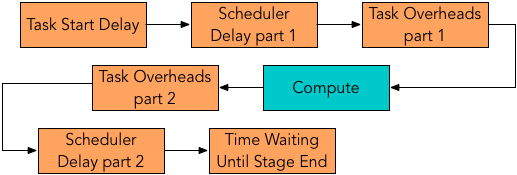
\includegraphics[width=.5\textwidth]{fig/spark_overheads.png}
\caption{Per task chronological breakdown of Spark overheads.}
\label{fig:overheads}
\end{center}
\end{figure}

\begin{itemize}[noitemsep,topsep=0mm]
  \item \emph{Task Start Delay}: the time between the stage start and when the driver sends the task to an executor.
  \item \emph{Scheduler Delay}: the sum of the time between when the task is sent to the executor and when it starts deserializing on the executor and the time between the completion of the serialization of the result of the task and the driver's reception of the task completion message.
  \item \emph{Task Overhead Time}: the sum of the fetch wait times, executor deserialize times, result serialization times, and shuffle write times.
  \item \emph{Time Waiting Until Stage End}: the time spent waiting on the final task in the stage to end.
\end{itemize}


